\documentclass{article}
\usepackage[utf8]{inputenc}
\usepackage{amsmath}
\usepackage[margin=1in]{geometry}
\usepackage[]{algorithm2e}
\usepackage{natbib}
\usepackage{multirow}
\usepackage{graphicx}
\usepackage{color}
\usepackage{todonotes}
\usepackage{booktabs,floatrow}
\newcommand{\comment}[1]{\textcolor{red}{SK: #1}}


\pagenumbering{arabic}
\setlength{\parindent}{0cm}

\DeclareMathOperator*{\argmax}{arg\,max}
\DeclareMathOperator*{\argmin}{arg\,min}

\title{ADMM Project Notes, Updated}
\author{Irina Tolkova}

\begin{document}

\maketitle

\tableofcontents

\section{Problem Description}

We aim to solve the problem in which a quadratic cost over the decision variable $y$ (states and inputs) is minimized under dynamic feasibility and other constraints:
\begin{align*}
\underset{y}{\text{minimize}} \; \; &y^T \bar{C} y + b^T y \\
\text{subject to} \; \; &f(y) = 0 \\
&g(y) = 0
\end{align*}

By linearizing the constraints around the previous trajectory, each iteration of this algorithm can be made into a convex problem. Define the matrices $M$ and $G$ such that
\[
M_{ij} = \frac{\partial f_i(y)}{\partial y_i} \;\;\; G_{ij} = \frac{\partial g_i(y)}{\partial y_i}
\]
and the vectors $c$ and $h$ which contain the residuals of the linearization from the previous solution (as defined in other notes document). Then, each iteration of this algorithm solves the problem
\begin{align*}
\underset{y}{\text{minimize}} \; \; &y^T \bar{C} y + b^T y \\
\text{subject to} \; \; &M y = c \\
&G y = h
\end{align*}

I had started with a penalty approach, and made the objective separable across terms with a consensus term. This resulted in the problem:
\begin{align*}
\underset{y}{\text{minimize}} \; \; &w^T \bar{C} w + b^T w + \frac{\rho_1}{2} ||My - c||_2^2 + \frac{\rho_2}{2} ||Gy - h||_2^2 \\
\text{subject to} \; \; &w = y
\end{align*}
which corresponds to the augmented Lagrangian:
\[
L(w, y) = w^T \bar{C} w + b^T w + \lambda_0 (w - y) + \frac{\rho_0}{2} ||w - y||_2^2 + \frac{\rho_1}{2} ||My - c||_2^2 + \frac{\rho_2}{2} ||Gy - h||_2^2
\]

Alternatively, if a separate dual term is associated with each constraint, the augmented Lagrangian would be
\begin{align*}
L(w, y) &= w^T \bar{C} w + b^T w \\
        &+ \lambda_0^T (w - y) + \lambda_1^T (My - c) + \lambda_2^T (Gy - h)\\
        &+ \frac{\rho_0}{2} ||w - y||_2^2 + \frac{\rho_1}{2} ||My - c||_2^2 + \frac{\rho_2}{2} ||Gy - h||_2^2
\end{align*}

\section{Variable Update Equations}

\subsection{Penalty Method}

The update for $w$ will be
\begin{align*}
w \leftarrow
&\argmin_w L(w, y) = \argmin_w \;\; [w^T (C + \frac{\rho_0}{2} I) w + w^T (\lambda_0 + b - \rho_0 y)] = \\
&(2C + \rho_0 I)^{-1} (\rho_0 y - \lambda_0 - b)\\
\end{align*}

The update for $y$ will be
\begin{align*}
y \leftarrow
&\argmin_y L(w, y) = \\
&\argmin_y \;\; [y^T (\frac{\rho_0}{2} I + \frac{\rho_1}{2} M^T M + \frac{\rho_2}{2} G^T G) y + y^T (-\lambda_0 - \rho_0 w - \rho_1 M^T c - \rho_2 G^T h)] = \\
&(\rho_0 I + \rho_1 M^T M + \rho_2 G^T G)^{-1}(\lambda_0 + \rho_0 w + \rho_1 M^T c + \rho_2 G^T h)
\end{align*}

There is only one dual variable corresponding to the consensus constraint, and its update is
\[
\lambda_0 \leftarrow \lambda_0 + \rho_0 (w - y)
\]

\subsection{Constrained Method}

The update for $w$ will be identical:
\begin{align*}
w \leftarrow (2C + \rho_0 I)^{-1} (\rho_0 y - \lambda_0 - b)\\
\end{align*}

The update for $y$ will have two extra terms ($M^T \lambda_1$ and $G^T \lambda_2$):
\begin{align*}
y \leftarrow
&\argmin_y L(w, y) = \\
&\argmin_y \;\; [y^T (\frac{\rho_0}{2} I + \frac{\rho_1}{2} M^T M + \frac{\rho_2}{2} G^T G) y + y^T (-\lambda_0 + M^T \lambda_1 + G^T \lambda_2 - \rho_0 w - \rho_1 M^T c - \rho_2 G^T h)] = \\
&(\rho_0 I + \rho_1 M^T M + \rho_2 G^T G)^{-1}(\lambda_0 - M^T \lambda_1 - G^T \lambda_2 + \rho_0 w + \rho_1 M^T c + \rho_2 G^T h)
\end{align*}

There are now three dual variables corresponding to each of the constraints, and the updates are
\begin{align*}
&\lambda_0 \leftarrow \lambda_0 + \rho_0 (w - y) \\
&\lambda_1 \leftarrow \lambda_1 + \rho_1 (My - c) \\
&\lambda_2 \leftarrow \lambda_2 + \rho_2 (Gy - h) \\
\end{align*}


\subsection{Slack Variables on Inequality Constraints}

In the above method, inequality constraints were treated as active or inactive based on the violation in the previous iteration. As a result, the Lagrange multipliers corresponding to inequality constraints would be incremented when the constraints were active, but not changed when they were inactive, causing them to "overshoot". To mitigate this issue, we can introduce slack variables following Nocedal and Wright (pg 514). \\

First, separate the matrix $G$ into $G_E$ and $G_I$, where the former corresponds to all equality constraints and the latter corresponds to all inequality constraints. The problem can be written as
\begin{align*}
\underset{y}{\text{minimize}} \; \; &w^T \bar{C} w + b^T w \\
\text{subject to} \; \; &w = y \\
&My - c = 0 \\
&G_E y - h_E = 0 \\
&G_I y - h_I + s = 0 \\
&s \geq 0
\end{align*}

Now, we can ((why?)) make a partial augmented Lagrangian, which is subject to the constraint $s \geq 0$:
\begin{align*}
L(w, y, s) &= w^T \bar{C} w + b^T w \\
        &+ \lambda_0^T (w - y) + \lambda_1^T (My - c) + \lambda_{2}^T (G_E y - h_E) + \lambda_{3}^T (G_I y - h_I + s)\\
        &+ \frac{\rho_0}{2} ||w - y||_2^2 + \frac{\rho_1}{2} ||My - c||_2^2 + \frac{\rho_2}{2} ||G_E y - h_E||_2^2 + \frac{\rho_3}{2} ||G_I y - h_I + s||_2^2
\end{align*}

While there are now more decision variables in the problem, the (constrained) minimization over $s$ has an analytic solution:
\begin{align*}
\argmin_s L(w, y, s)
&= \argmin_s \;\; [ \lambda_{3}^T s + \frac{\rho_3}{2} ||G_I y - h_I + s||_2^2] = \\
&= \argmin_s \;\; [ \lambda_{3}^T s + \frac{\rho_3}{2} s^T s + \rho_3 s^T (G_I y - h_I)]
\end{align*}

The unconstrained solution can be found by setting the derivative to zero:
\begin{align*}
\rho_3 s + \rho_3 (G_I y - h_I) + \lambda_3 = 0
\;\; \rightarrow \;\;
s = -\frac{\lambda_3}{\rho_3} - (G_I y - h_I)
\end{align*}

Since this is a (convex) minimization of a quadratic for each constraint, if an element $s_i$ of the solution vector does not satisfy the non-negativity constraint, the solution will occur at $s_i = 0$. Overall,
\[
s = \text{pointwise maximum}(-\frac{\lambda_3}{\rho_3} - (G_I y - h_I), 0)
\]

If this is substituted into the augmented Lagrangian, we get
\begin{align*}
L(w, y) &= w^T \bar{C} w + b^T w + \lambda_0^T (w - y) + \lambda_1^T (My - c) + \lambda_{2}^T (G_E y - h_E) \\
&+ \frac{\rho_0}{2} ||w - y||_2^2 + \frac{\rho_1}{2} ||My - c||_2^2 + \frac{\rho_2}{2} ||G_E y - h_E||_2^2 \\
&+ \sum_{i \in I} \;\phi_i(y)
\end{align*}
where
\[
\phi_i(y) =
\left(\begin{array}{ll}
\lambda_{3}^T (G_i y - h_i) +  \frac{\rho_3}{2} ||G_i y - h_i||_2^2 & \text{if  } -\frac{\lambda_3}{\rho_3} \leq (G_I y - h_I) \\
-\frac{\lambda_{3, i}^2}{2 \rho_3} & \text{if  } -\frac{\lambda_3}{\rho_3} > (G_I y - h_I)
\end{array}\right)
\] 

We can show that the dual update will be the same as before, but thresholded to zero:
\[
\lambda_i^{k+1} = \max(\lambda_i^k + \rho_3 (G_i y - h_h), 0)
\]

To find the updates for ADMM, we could choose one of the two cases for each point based on the value of the constraint in the previous iteration, and minimize with respect to $y$. This is actually very similar to the more naive update that had been applied previously, which would have used the function
\[
\phi_i(y) =
\left(\begin{array}{ll}
\lambda_{3}^T (G_i y - h_i) +  \frac{\rho_3}{2} ||G_i y - h_i||_2^2 & \text{if  } 0 \leq (G_I y - h_I) \\
0 & \text{if  } 0 > (G_I y - h_I)
\end{array}\right)
\] 

Essentially, the slack variable approach adds a buffer on both the primal and dual update for inequality constraints, such that they are updated even if the constraint is satisfied (within a range defined by $\lambda_3$ and $\rho_3$). \\

We can test this inequality thresholding method on a toy problem to see its effects. For instance, consider the problem with two 1-dimensional decision variables (x, y):
\begin{align*}
\underset{x, y}{\text{minimize}} \; \; &2 x^2 + 2 y^2 + 2x + y \\
\text{subject to} \; \; &y^2 \leq x \\
&x \leq y^2/4 - 2
\end{align*}

Figure \ref{toy_admm_iterations_1} shows the path of the two consensus variables across iterations of ADMM, in which the constraint vector and gradients are thresholded to 0 if the constraints are not violated. There is a large oscillation in the points as a result of conflicting pulls from the constraint and the objective. This oscillation is also visible in plots of the norms of the Lagrange multipliers across iterations (Figure \ref{toy_admm_iterations_1}). However, if the buffer term is added, the trajectory and the norms become smooth, as shown in Figures \ref{toy_ali_iterations_1}, \ref{toy_ali_norms_1}. All other values/parameters were kept the same. Note that the final solution is feasible even though the second Lagrange multiplier converges to a nonzero value. \\

If the center of the objective function was to the other side of the feasible region, there is similar behavior. Figures \ref{toy_admm_iterations_2} and \ref{toy_admm_norms_2} show the results of ADMM, and Figures  \ref{toy_ali_iterations_2} and \ref{toy_ali_norms_2} show the results of ALI. However, it looks like ALI can still diverge due to oscillation if the first penalty parameter (associated with the consensus constraint) is set too low relative to the second penalty parameter (associated with the two explicit constraints).

\begin{figure}
\begin{tabular}{cc}
  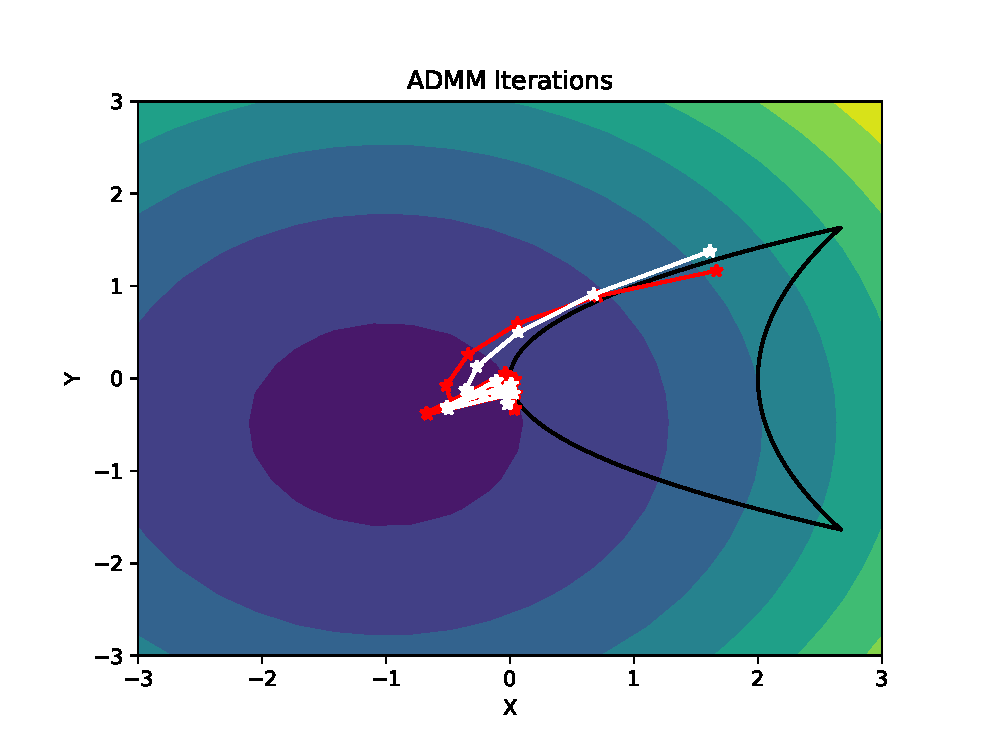
\includegraphics[width=80mm]{figures/toy_admm_iterations_1.eps} &   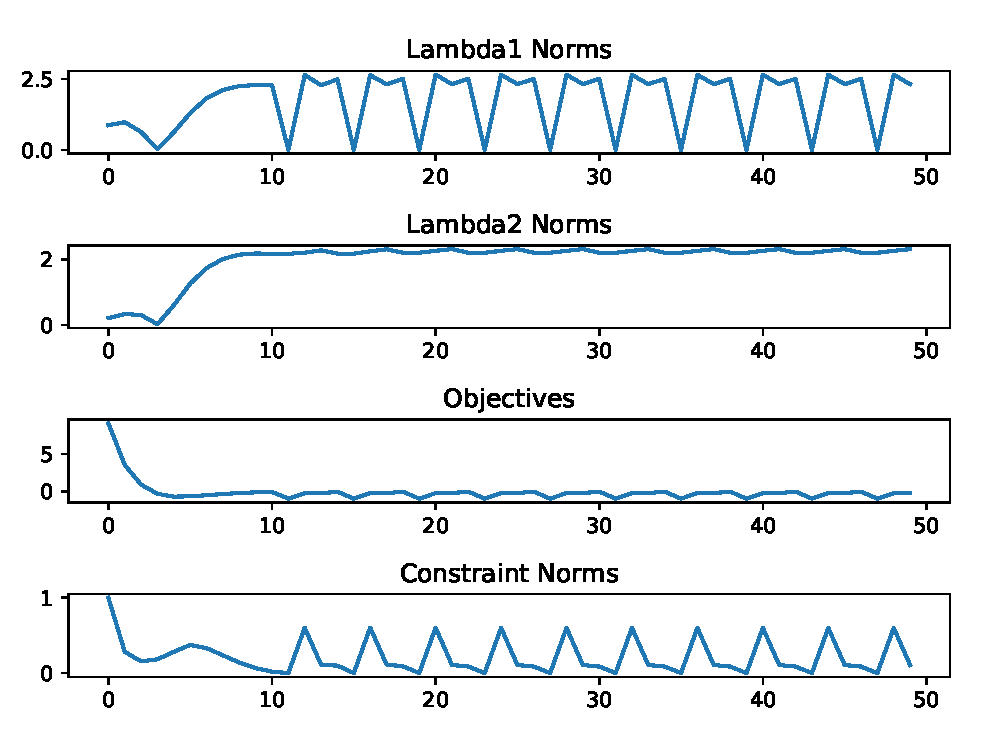
\includegraphics[width=80mm]{figures/toy_admm_norms_1.eps} \\
 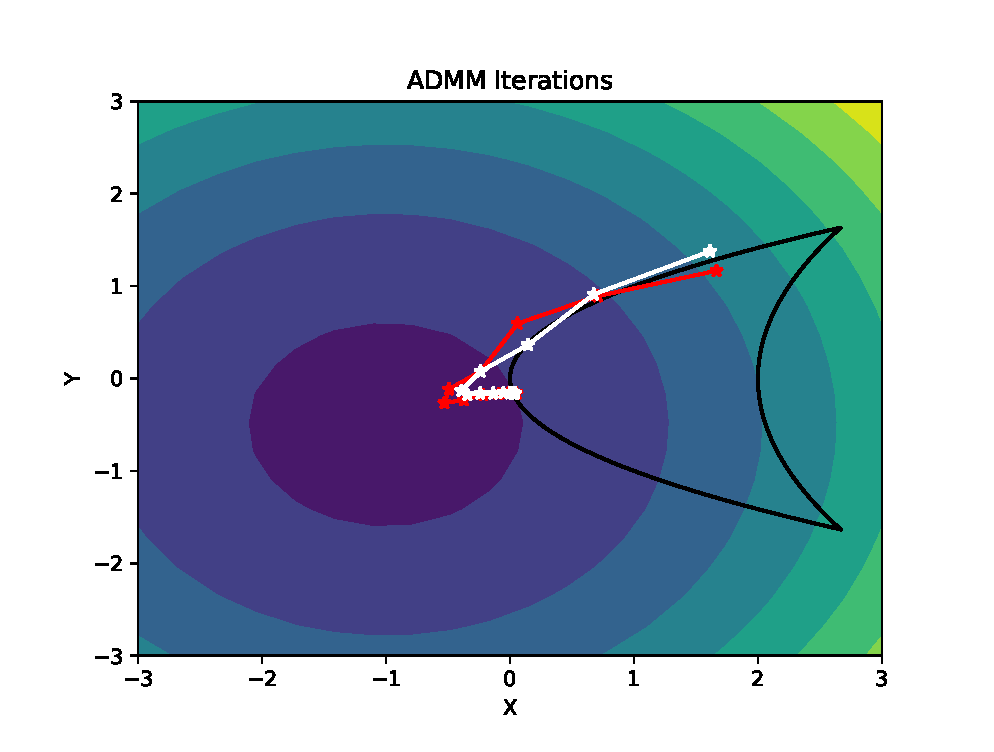
\includegraphics[width=85mm]{figures/toy_ali_iterations_1.eps} &   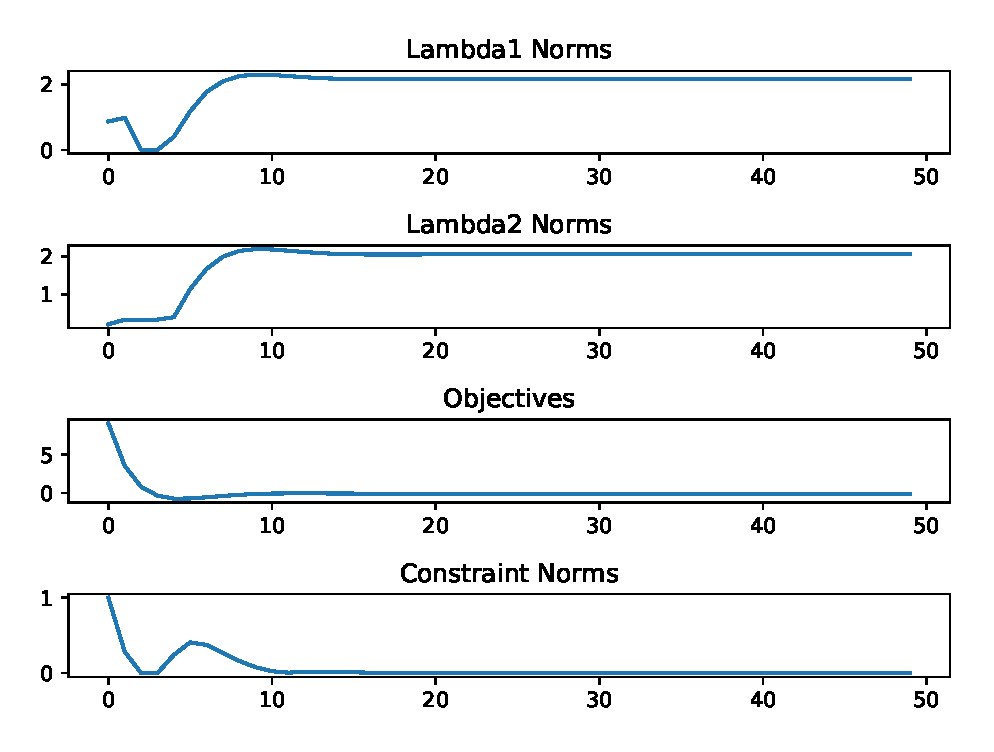
\includegraphics[width=85mm]{figures/toy_ali_norms_1.eps} \\
\end{tabular}
\caption{caption}
\label{fig:quad_trajectories}
\end{figure}

\begin{figure}
\begin{tabular}{cc}
  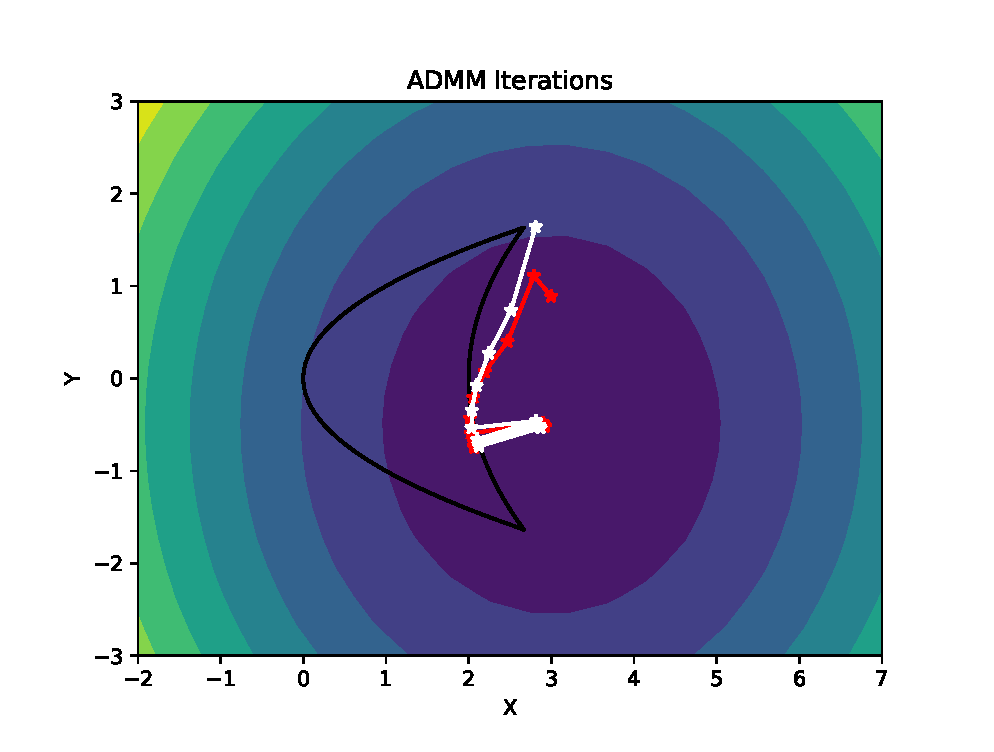
\includegraphics[width=80mm]{figures/toy_admm_iterations_2.eps} &   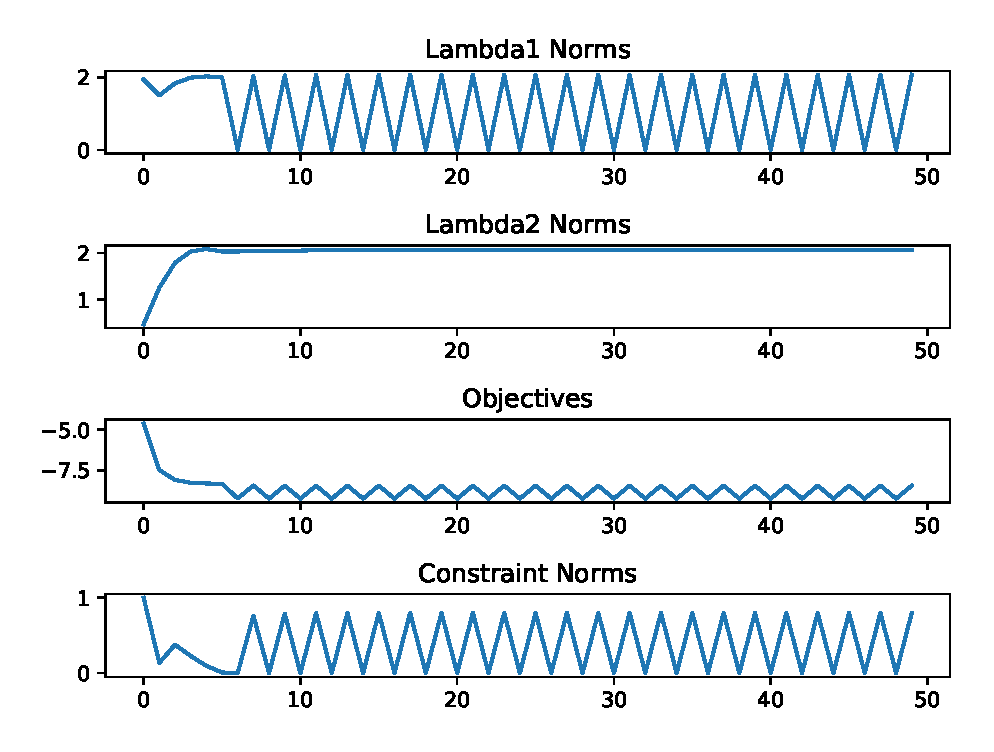
\includegraphics[width=80mm]{figures/toy_admm_norms_2.eps} \\
 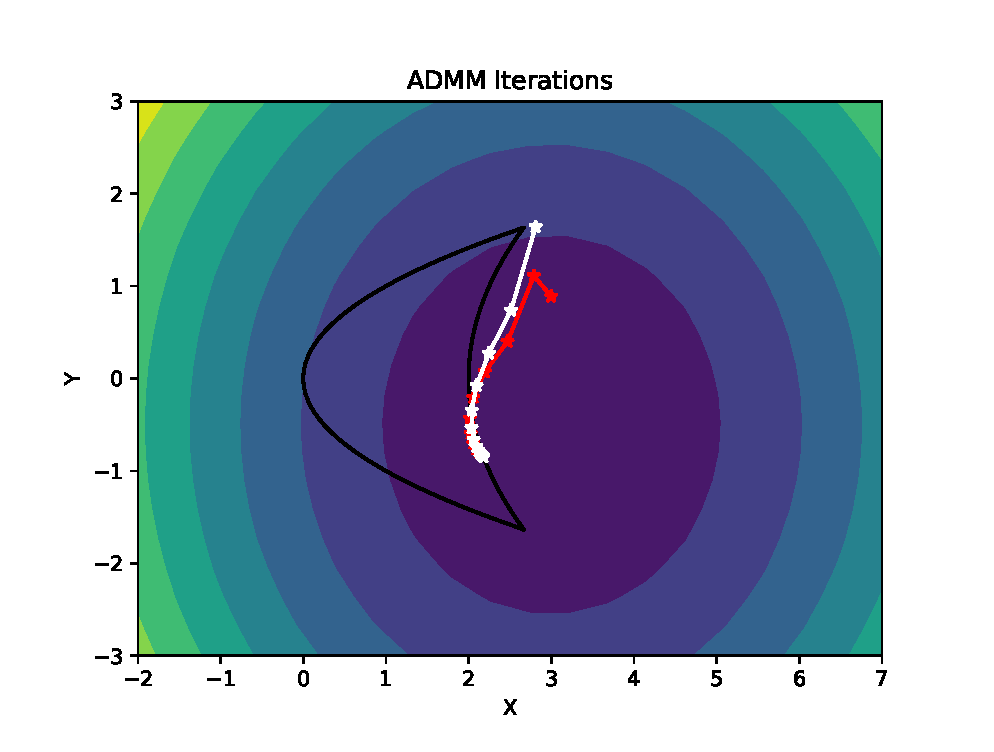
\includegraphics[width=85mm]{figures/toy_ali_iterations_2.eps} &   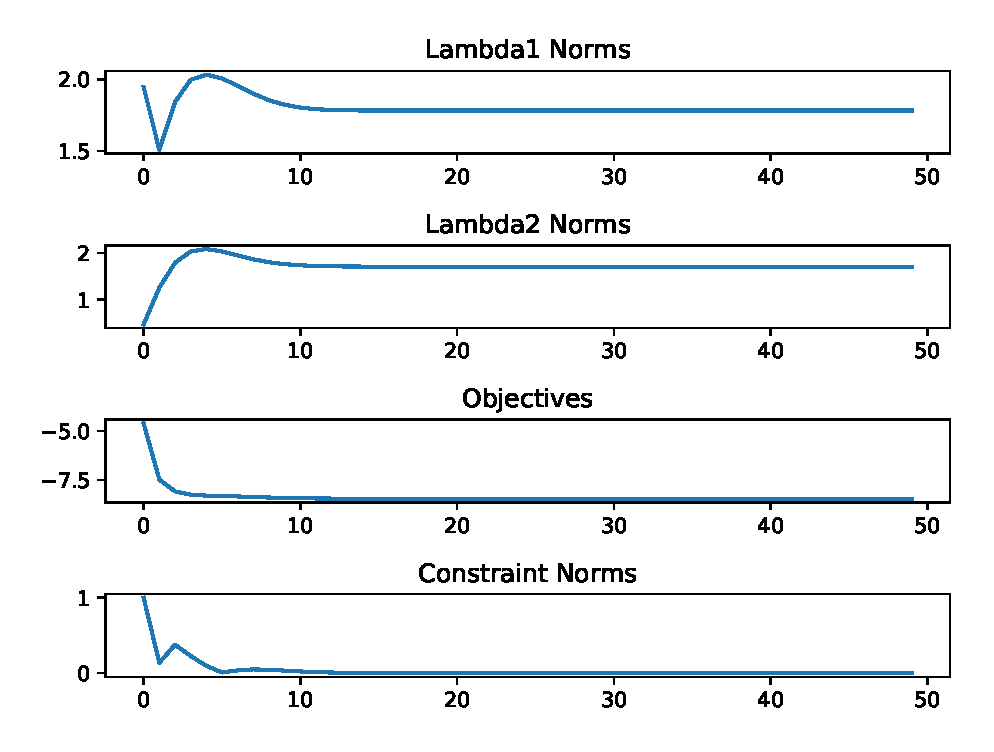
\includegraphics[width=85mm]{figures/toy_ali_norms_2.eps} \\
\end{tabular}
\caption{caption}
\label{fig:quad_trajectories}
\end{figure}


\end{document}
